% =====================================================================
%  chunks/ch02a.tex —— 原书 p.15–22（PDF 22–29）
%  第 2 章 拓扑空间. 纤维化. 同伦
%  §1 一般拓扑的观察与术语；§2 同伦. 同伦型；§3 覆叠同伦. 纤维化（开头）
%  注：原书 p.15 顶部一段是第 1 章末例子的收尾，按分工由 ch01 写到 p.15；本块从章标题开始。
% =====================================================================
% [原文 p.15]
\chapter{拓扑空间。纤维化。同伦}

\section{一般拓扑的观察与术语}

\takeaway{拓扑结构只由「哪些子集算开集」给定：连续、紧、Hausdorff、道路连通、乘积拓扑与紧开拓扑、楔和、映射柱、子空间、序列收敛、同胚、流形，全都可用开集与映射表述。本节引入的 $\pi_0$、$Y^X$、$X\vee Y$、$C_f$ 等记号在全书反复出现。}

尽管拓扑性质有时藏在一副组合–代数的面具之后，它们却无一例外地都属于连续性这一概念。集合之间的连续映射（或连续函数）的最一般定义，对集合上所需的结构要求极少。按 Fréchet 的提法，集合 $X$ 上的这种结构（或拓扑）——它使 $X$ 成为一个\emph{拓扑空间}——仅仅在于指定 $X$ 的某些子集 $U$（在 $X$ 的全部子集之中）作为 $X$ 的\emph{开集}；要求只有两条：空集与全空间 $X$ 是开集；全体开集之集对以下运算封闭——任意有限多个开集的交仍是开集，任意多个（有限或无限）开集的并仍是开集。开集 $U$ 的补集 $X\setminus U$ 称为\emph{闭集}。子集 $V\subset X$ 的\emph{闭包}记作 $\bar V$，是包含 $V$ 的最小闭集。拓扑空间 $X$ 与 $Y$ 之间的\emph{连续映射}（简称\emph{映射}）$f:X\to Y$，是指这样的映射：$Y$ 的每个开集 $U$ 的完全原像 $f^{-1}(U)$ 都是 $X$ 的开集。（任意子集 $D\subset Y$ 的完全原像 $f^{-1}(D)$，就是一切满足 $f(x)\in D$ 的 $x\in X$ 之集。）\emph{紧}空间是这样的拓扑空间 $X$：任给 $X$ 的一个由开集 $U_\alpha$ 组成的覆盖，即 $\bigcup_\alpha U_\alpha=X$，总存在有限个指标 $\alpha_1,\dots,\alpha_N$，使开集 $U_{\alpha_1},\dots,U_{\alpha_N}$ 已经覆盖 $X$，亦即总存在有限子覆盖。可以证明，在紧空间 $X$ 中，每个点列 $x_i$，$i=1,2,\dots$，都在 $X$ 中有极限点 $x_\infty$；也就是说，每个包含 $x_\infty$ 的开集都含有该点列的无穷多个项 $x_i$。
% [Tutor Note: 原书此句对一般拓扑空间并不成立：紧性推出「每个点列有聚点」需要空间第一可数（或改用滤子、网来表述紧性）。本书随后就把注意力放在度量空间与 CW 复形上，那里第一可数自动成立，所以作者不加条件。]

\emph{Hausdorff} 拓扑空间是指具有下述性质的拓扑空间：对任意两个不同的点 $x_1,x_2$，存在互不相交的开集 $U_1,U_2$ 分别包含它们，即 $U_1\cap U_2=\varnothing$，$x_1\in U_1$，$x_2\in U_2$。拓扑空间 $X$ 称为\emph{度量空间}，若对每对点 $x_1,x_2\in X$ 都定义有一个实值「距离」$\rho(x_1,x_2)$，它关于 $x_1,x_2$ 连续（相对于 $X\times X$ 上的「乘积拓扑」——见下文），并且满足
\begin{align*}
% [原文 p.16]
  &\rho(x_1,x_2)>0\quad\text{若 }x_1\ne x_2,\\
  &\rho(x,x)=0,\qquad \rho(x_1,x_2)=\rho(x_2,x_1),\\
  &\rho(x_1,x_2)+\rho(x_2,x_3)\ge\rho(x_1,x_3).
\end{align*}

度量空间总是 Hausdorff 的。\emph{道路连通}空间 $X$ 是指其中任意两点 $x_1,x_2$ 都能用 $X$ 中的一条连续道路连接；所谓\emph{道路}，是区间 $I$ 到 $X$ 的一个映射 $I\to X$。每个拓扑空间都分解为两两不相交的极大道路连通分支（\emph{道路分支}）。$X$ 的道路分支之集记作 $\pi_0(X)$，称为 $X$ 的「同伦群的零维类比物」；一般说来，这个集合并不带自然的群结构，只有在某些特殊（且重要）的情形下才带（见下）。
% [Tutor Note: $\pi_0$ 只是集合，没有群运算；它与高阶同伦群 $\pi_n$（$n\ge 1$ 是群，$n\ge 2$ 是交换群）的类比仅在于「把空间映成代数对象」这一思路。后文 §4 会用 $\pi_0$ 记纤维化纤维的道路分支集，切勿与同伦群混为一谈。]

给定拓扑空间 $X,Y$，可以构造它们的\emph{直积} $X\times Y$：其点是序对 $(x,y)$，$x\in X$，$y\in Y$；其拓扑以形如 $U\times V$ 的子集为「基」，其中 $U$ 是 $X$ 的开集，$V$ 是 $Y$ 的开集。（$X\times Y$ 的任意开集于是由任意多个基本开集取并得到。）给定拓扑空间 $X,Y$，人们通常给全体连续映射 $f:X\to Y$ 之集 $Y^X$ 赋以一种拓扑，称为\emph{紧开拓扑}。定义如下：取 $X$ 的任意紧子集 $K$ 与 $Y$ 的任意开集 $V$；一切把 $K$ 映入 $V$（即 $f(K)\subset V$）的映射 $f$ 之集，就是 $Y^X$ 的一个典型基本开集。若空间 $X$ 本身紧、$Y$ 是带度量 $\rho$ 的度量空间，则 $Y^X$ 是度量空间，其度量 $\tilde\rho$ 由
\[
  \tilde\rho(f,g)=\max_{x\in X}\rho(f(x),g(x)),\qquad f,\ g:X\to Y
\]
给出。

还有由一对拓扑空间 $X,Y$ 出发的另一个简单而重要的构造，即它们的\emph{楔和} $X\vee Y$。严格说来，楔和是对\emph{带点空间} $X,Y$ 定义的，即指定了基点 $x_0\in X$、$y_0\in Y$ 的空间；它们的楔和 $X\vee Y$，是把 $X$ 与 $Y$ 的形式不交并中的 $x_0$ 与 $y_0$ 粘合（$x_0\approx y_0$）所得的商空间：
\begin{figure}[htbp]
  \centering
  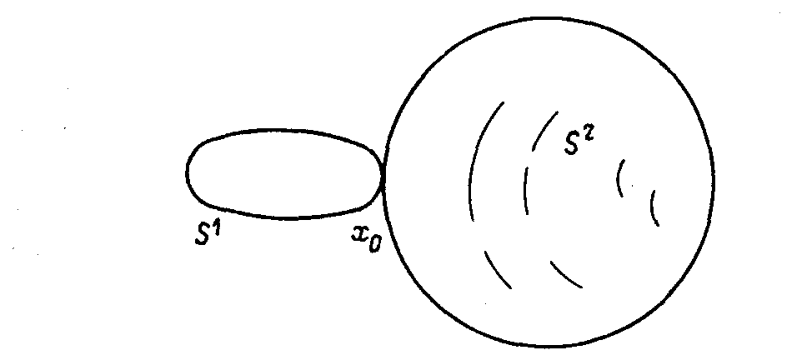
\includegraphics[width=0.52\textwidth]{figures/fig2_1.png}
  \figtitle{2.1}{楔和 $X\vee Y$}
\end{figure}
% [原文 p.17]
\begin{equation}
  X\vee Y=X\dot\cup Y/x_0\approx y_0. \tag{1.1}
\end{equation}

更一般地，给定任意闭子集 $A\subset X$ 与映射 $f:A\to Y$，可以用粘合手段构造楔和的如下类比：
\[
  X\vee_{(A,f)}Y=X\dot\cup Y/x\approx f(x),\quad x\in A.
\]
其重要特例是映射 $f:Z\to Y$ 的\emph{映射柱} $C_f$。考虑 $Z$ 与区间 $I=[a,b]$ 的乘积，作粘合空间
\begin{equation}
  C_f=(Z\times I)\dot\cup Y/(z,b)\approx f(z),\quad z\in Z. \tag{1.2}
\end{equation}
（这里 $Z\times I$ 充当 $X$，$Z\times\{b\}$ 充当 $A$。）$C_f$ 上的拓扑按自然方式定义：$C_f$ 的子集取作开集，当且仅当它在自然映射 $Z\times I\to C_f$ 与 $Y\to C_f$ 下的完全原像都是开集。
% [Tutor Note: 映射柱把 $f$ 换成一对包含映射：$Z\simeq Z\times I$ 与 $Y$ 都嵌入 $C_f$，且 $Z\hookrightarrow C_f$ 是余纤维化。第 3 章构造 CW 复形时，粘合映射的映射柱就是把胞腔粘上去的严格写法。]

在拓扑空间 $X$ 的任意子集 $A$ 上，\emph{子空间拓扑}（或\emph{诱导拓扑}）定义为：把 $A$ 的开集取作 $X$ 的开集与 $A$ 的交。

若拓扑空间 $X$ 的点列 $x_i$ 在 $X$ 中有极限，即存在点 $x_\infty\in X$，使每个包含 $x_\infty$ 的开集 $U$ 都含有几乎所有的 $x_i$（即除有限多个之外的所有 $x_i$），则称该点列在 $X$ 中\emph{收敛}。由收敛点列的知识可以还原 $X$ 上的拓扑。

拓扑空间 $X$ 与 $Y$ 之间的\emph{同胚}，是连续的一一满射 $f:X\to Y$，并且其逆 $f^{-1}:Y\to X$ 也连续。这里，逆函数 $f^{-1}$ 的连续性一般不能由其余定义条件推出；但当 $X$ 紧、$Y$ 是 Hausdorff 空间时，它确实可以推出。
% [Tutor Note: 这一句的论证是闭映射：紧空间到 Hausdorff 空间的连续映射把闭集映成闭集；于是连续双射的逆把闭集映成闭集，故逆连续。原书只说「可以推出」，略去的正是「紧 $\Rightarrow$ 闭映射」这一步。]

泛函分析提供了许多连续双射而其逆不连续的例。特别地，对实值光滑函数空间，按不同阶数的导数可以定义各种自然的收敛方式；因此即使在这样相对具体的框架里，出现逆不连续的连续双射也是意料之中的。

人们常遇到同时带有某种代数结构的拓扑空间，这种结构与拓扑结构相容，意思是各种代数运算作为映射都连续；于是有\emph{拓扑群}、\emph{拓扑向量空间}、\emph{拓扑环}等等。

从纯抽象的观点看，考虑具有局部欧氏性质的拓扑空间是非常自然的；不过实际上，这类对象最常自然出现时，还连带某种额外的光滑结构或分片线性结构（PL 结构）。

\begin{definition*}{1.1}
（$n$ 维的）\emph{拓扑流形}是指这样的 Hausdorff 拓扑空间 $X$：它的每个点 $x$ 都有一个开邻域 $U$（即包含 $x$ 的开集，或称「区域」），
它同胚于 $n$ 维欧氏空间 $\R^n$ 的某个开集（$n$ 固定）。
% [原文 p.18]
\end{definition*}
% [Tutor Note: 定义只要求 Hausdorff 与局部欧氏，没有要求第二可数或仿紧：若不加可数性，「长直线」也满足此定义却不是通常意义下的流形。本书后文默认所论流形仿紧（故可嵌入某个 $\R^N$），读者宜记住这一隐含前提。]

于是 $n$ 维流形被一些开集 $U_\alpha$ 覆盖，每个 $U_\alpha$ 同胚于 $\R^n$；因此经由某个具体的同胚 $\varphi:U_\alpha\to\R^n$，每个 $U_\alpha$ 上诱导出\emph{局部坐标} $x_\alpha^1,\dots,x_\alpha^n$。在每个重叠区域 $U_\alpha\cap U_\beta$ 上，于是定义了两套（或更多套）局部坐标，从而有从其中一套到另一套的坐标变换：
\[
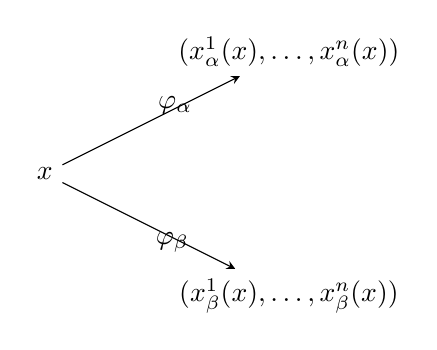
\begin{tikzpicture}[>=stealth,baseline=(x.base)]
  \node (x) at (0,0) {$x$};
  \node (xa) at (3.1,1.55) {$(x_\alpha^1(x),\dots,x_\alpha^n(x))$};
  \node (xb) at (3.1,-1.55) {$(x_\beta^1(x),\dots,x_\beta^n(x))$};
  \draw[->] (x) -- node[above right=-1pt] {$\varphi_\alpha$} (xa);
  \draw[->] (x) -- node[below right=-1pt] {$\varphi_\beta$} (xb);
\end{tikzpicture}
\]
\begin{equation}
  \begin{gathered}
    x_\alpha^j=f_\alpha^j(x_\beta^1,\dots,x_\beta^n),\qquad
    x_\beta^k=g_\beta^k(x_\alpha^1,\dots,x_\alpha^n),\\
    f\circ g=1.
  \end{gathered}
  \tag{1.3}
\end{equation}

\section{同伦。同伦型}

\takeaway{同伦是「映射可以连续形变」的形式化：一个同伦就是 $X\times I\to Y$ 的连续映射。同伦等价、形变收缩、可缩性都由「同伦于恒等映射」刻画，故同伦型比同胚型粗；映射的同伦类恰是函数空间 $Y^X$ 的道路分支。}

映射 $f:X\to Y$ 的\emph{连续同伦}（简称\emph{同伦}或\emph{形变}），是柱体 $X\times I$ 到 $Y$ 的一个连续映射
\[
  F=F(x,t):X\times I\to Y,\quad x\in X,\ a\le t\le b
\]
（其中 $I$ 是区间 $[a,b]$），使得对一切 $x\in X$ 有
\[
  F(x,a)=f(x).
\]
两个映射 $f,g:X\to Y$ 称为\emph{同伦的}，若存在连续同伦 $F$ 使
\[
  F(x,a)=f(x),\quad F(x,b)=g(x),\quad x\in X.
\]

在这种讨论中常常需要考虑\emph{带点空间} $X,Y$，即指定了特殊点 $x_0\in X$、$y_0\in Y$ 的空间。对这种空间，映射 $f:X\to Y$ 通常还要求是「带点的」，即满足 $f(x_0)=y_0$；而「带点」映射之间的同伦也照例要求是「带点的」，意思是对一切 $t$ 有 $F(x_0,t)=y_0$。

同伦映射 $f:X\to Y$ 的每个等价类都构成函数空间 $Y^X$ 的一个道路分支，称为映射 $X\to Y$（或带点映射，视情形而定）的\emph{同伦类}。于是集合 $\pi_0(Y^X)$ 恰由同伦类组成。
% [Tutor Note: 「同伦类 = $Y^X$ 的道路分支」这一等同依赖于 $Y^X$ 上的紧开拓扑与 $I$ 的紧性：$X\times I\to Y$ 的连续映射与 $I\to Y^X$ 的连续映射一一对应（指数律）。后面 §4 把同伦类记作 $[X,Y]$，并证明它与 $\pi_0(Y^X)$ 一致。]

有时还必须处理空间对 $A\subset X$、$B\subset Y$，此时所论的映射 $f:X\to Y$ 是满足 $f(A)\subset B$ 的映射。这样的\emph{空间对的映射}记作
\[
  f:(X,A)\to(Y,B),
\]
而全体这样的空间对映射之空间，其道路分支就是空间对映射的相应同伦类。下文将会看到，有几条重要理由要求再考虑三元组 $(x_0\in A\subset X)$ 的范畴：此时所论的映射 $f:X\to Y$ 要求同时满足 $f(A)\subset B$ 与 $f(x_0)=y_0$，其中 $(y_0\in B\subset Y)$ 是另一个这样的三元组。这里得到的是空间对带点映射的同伦类。
% [原文 p.19]

\begin{definition*}{2.1}
连续映射 $f:X\to Y$ 称为\emph{同伦等价}，若存在「同伦逆」映射 $g:Y\to X$，使得两个复合 $g\circ f:X\to X$ 与 $f\circ g:Y\to Y$ 分别同伦于相应的恒等映射
\[
  1_X:X\to X\quad(1_X(x)\equiv x),\qquad 1_Y:Y\to Y\quad(1_Y(y)\equiv y).
\]
\end{definition*}
（对带点空间，按显然的方式修改此定义，就得到\emph{带点同伦等价}的概念。）此时称空间 $X,Y$ \emph{同伦等价}，记作 $X\sim Y$，或称它们具有\emph{相同的同伦型}。

现在设以下条件成立：$X$ 是 $Y$ 的子空间（或嵌入 $Y$ 中）；$f:X\to Y$ 是包含映射；$g:Y\to X$ 限制在 $X$ 上是 $X$ 上的恒等映射；最后，在把 $f\circ g:Y\to Y$ 形变为恒等映射 $1_Y$ 的整个同伦 $F$ 中，对一切 $x\in X\subset Y$ 都有 $F(x,t)=x$。在这种情形下，子空间 $X$ 称为 $Y$ 的\emph{形变收缩}。例如 $\R^n$ 的任意开区域 $Y$ 都有维数更低的形变收缩。整个欧氏空间 $\R^n$ 以任意一点为其形变收缩。具有后一性质的空间 $Y$ 称为\emph{可缩的}（相对于自身），或称\emph{同伦平凡的}：$Y\sim 0$。
% [Tutor Note: 「$Y\sim 0$」中的 $0$ 指点空间（单点空间），不是空集。可缩等价于 $Y$ 同伦等价于单点，也等价于恒等映射 $1_Y$ 同伦于常映射。注意形变收缩比收缩强：它要求整个形变过程中 $X$ 上点点不动。]

空间 $Y$ 到其子空间 $X\subset Y$ 上的\emph{收缩}，是映射 $f:Y\to X$，使 $f$ 限制在 $X$ 上是 $X$ 上的恒等映射：$f|_X=1_X$。此时称空间 $X$ 为 $Y$ 的\emph{收缩核}。

\section{覆叠同伦。纤维化}

\takeaway{纤维化是把底空间的同伦「整体提升」到全空间的映射（覆叠同伦性质）。覆叠空间与 Serre 纤维化是最基本的两个例子；同一道路连通分支上的纤维彼此同伦等价，这是后文用纤维作归纳的基础。}

考虑一个（连续）映射 $p:X\to Y$。称任意映射 $f:Z\to Y$ 被\emph{覆叠}（经由 $p$），若存在映射 $g:Z\to X$ 使 $f=p\circ g$。

现在设给定同伦 $F:Z\times I\to Y$，其中 $I=[a,b]$，并且在初始时刻 $t=a$，映射 $f(z)=F(z,a)$ 已被某个映射 $g:Z\to X$ 覆叠。

\begin{definition*}{3.1}
映射 $p:X\to Y$ 称为\emph{纤维化}，若任给空间 $Z$ 与任给同伦 $F:Z\times I\to Y$，只要其初始映射 $f(z)=F(z,a):Z\to Y$ 被覆叠（设由 $g(z)$ 覆叠），则整族同伦 $F$（它在下面 $Y$ 中）就被 $X$ 中某个同伦 $G:Z\times I\to X$ 在上面覆叠，即
\[
  p\circ G(z,t)=F(z,t).
\]
同伦 $G$ 称为 $F$ 的（以 $g$ 为初始映射的）\emph{覆叠同伦}。
% [原文 p.20]
\end{definition*}
% [Tutor Note: 定义要求对「任意空间 $Z$」成立，条件很强。若只对 CW 复形（或胞腔复形）$Z$ 要求，得到的是 Serre 纤维化；若进一步要求 $G$ 在 $F$ 固定的子区间上不动（见下段），得到的是 Hurewicz 纤维化。三者强弱不同，后文 §4 的正合列对 Serre 纤维化已足够。]

出于各种技术上的理由，在空间 $Z$ 带有这种或那种条件（例如胞腔性——见第 3 章）的场合，常采用本定义的一个减弱形式。不过纤维化这一概念的本质特征不会因这种改动而改变。

通常还在上述定义中附加如下条件：若点 $z_1\in Z$ 在 $[a,b]$ 的某个子区间上对一切 $t$ 都被同伦 $F(z,t)$ 固定，则它在同一子区间上也应被 $G(z,t)$ 固定。

在最重要的场合，覆叠同伦的构造借助「同伦联络」实现。粗略地说，\emph{同伦联络}是这样一种处方：给定 $Y$ 中从 $y_0\in Y$ 出发的一条道路，以及 $X$ 中位于 $y_0$ 上方的任意指定点 $x_0$，它给出 $X$ 中从 $x_0$ 出发的唯一一条覆叠道路。此外，这条覆叠道路应当连续依赖于 $Y$ 中给定的道路与覆叠道路的起点 $x_0\in X$ 两者；这就保证了覆叠同伦性质对所有性质足够好的空间 $Z$ 成立。
\begin{figure}[htbp]
  \centering
  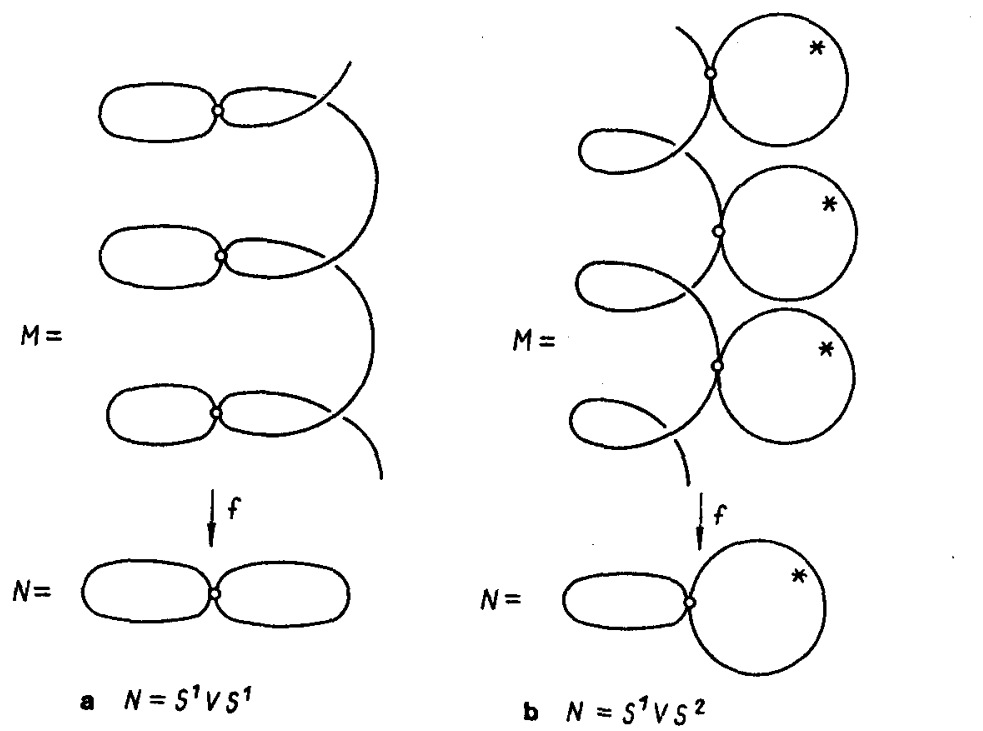
\includegraphics[width=0.72\textwidth]{figures/fig2_2.png}
  \figtitle{2.2}{}
\end{figure}

还有一些术语：给定纤维化 $p:X\to Y$，称 $p$ 为\emph{投影}，$X$ 为\emph{全空间}，$Y$ 为\emph{底空间}，而每个空间 $F_y=p^{-1}(y)$（$y\in Y$）为纤维化的一个\emph{纤维}。

取 $Z$ 为纤维化 $p:X\to Y$ 的一个纤维 $F_{y_0}$，$g:Z\to X$ 为包含映射，$f:Z\to Y$ 为把 $Z=F_{y_0}$ 映到单点
$y_0\in Y$ 的投影。设 $\gamma(t)$ 是 $Y$ 中连接 $y_0$ 与任意另一点 $y_1$ 的道路。利用覆叠同伦性质（以上述「同伦联络」的形式，我们总假定它存在），容易建立下述重要事实：\emph{$Y$ 的同一道路连通分支上的所有纤维 $F_y$ 都同伦等价}。事实上，此后我们总假定纤维化的底空间 $Y$ 道路连通。
% [原文 p.21]
% [Tutor Note: 这里「容易建立」用的是同伦联络：沿道路 $\gamma$ 把 $F_{y_0}$ 中的点同时搬过去，得到 $F_{y_0}\to F_{y_1}$ 的映射；沿反向道路搬回来与之复合，再由同伦联络的连续性（且提升唯一）得到同伦于恒等。之所以要求底空间道路连通，是为了保证不同纤维之间真有道路可沿。]

下面是最简单的几个例子。

\para{1. 覆叠空间} 映射 $p:X\to Y$ 称为\emph{覆叠映射}，$X$ 称为 $Y$ 的\emph{覆叠空间}，若它是带离散纤维 $F$ 的纤维化，即这样一个空间：它的所有子集都是开集（于是它的点——数目可以无限——彼此都是孤立的），并且对每个点 $y\in Y$ 都存在开邻域 $U$（$y\in U\subset Y$），其完全原像 $p^{-1}(U)$ 同胚于直积 $U\times F$，其中 $F=\bigcup_\alpha\{x_\alpha\}$：
\[
  p^{-1}(U)=\bigcup_\alpha U_\alpha\cong U\times F,
\]
这里每个 $U_\alpha\subset X$ 都是 $U$ 的同胚副本。诸 $U_\alpha$ 是 $X$ 的开集，$p$ 在每个 $U_\alpha$ 上的限制 $p|_{U_\alpha}:U_\alpha\to U$ 是与 $U$ 的同胚。对覆叠空间，同伦联络的存在性容易建立。
\begin{figure}[htbp]
  \centering
  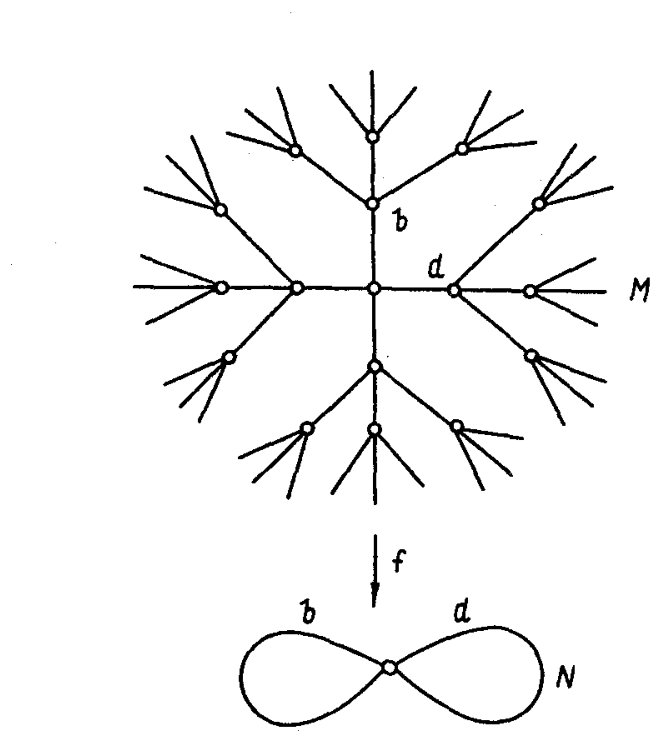
\includegraphics[width=0.34\textwidth]{figures/fig2_3.png}
  \figtitle{2.3}{}
\end{figure}
{\small 图中注记：这里覆叠空间是一棵无限的「十字」树（无圈，因而可缩）。每个顶点有四条边与之相接。\par}
% [Tutor Note: 原书 p.21 此句 "i.e a space all of those subsets are open" 英文有脱漏，意思应为「它的所有子集都是开集」，即 $F$ 上取离散拓扑；译按此意补足。另注意 $p^{-1}(U)$ 的各个 $U_\alpha$ 彼此不交，称为该覆叠在 $U$ 上的「叶」(sheet)，这正是 $U\times F$ 中每个 $U\times\{x_\alpha\}$ 的像。]

关于 $\R^2$ 的区域上的覆叠空间，第 1 章结合 Riemann 面已讨论过一些具体例子。在那些例子里，同伦联络是按显然的方式构造的。更多的例子见 图 2.2 与图 2.3。
% [原文 p.22]
\para{2. Serre 纤维化} 设 $B\subset Y$ 是任意一对空间，用 $X$ 记由 $Y$ 中始于 $B$ 的一切道路 $\gamma:[a,b]\to Y$ 组成的空间：
\[
  \gamma(a)\in B,\quad \gamma(b)\in Y,\quad \gamma\in X.
\]
考虑由
\[
  p(\gamma)=\gamma(b)
\]
定义的求值映射 $p:X\to Y$。这就定义了一个 \emph{Serre 纤维化} $p:X\to Y$。

为看出 $p:X\to Y$ 确实是纤维化，考虑底空间 $Y$ 中任意一条道路 $y(\tau)$，$b\le\tau\le c$，它始于给定道路 $\gamma\in X$ 的终点，$y(b)=\gamma(b)$。对曲线 $y(\tau)$ 的每个点 $y$，把从 $y(b)$ 到 $y(\tau)=y$ 的那一段接到 $\gamma$ 上，得到道路 $\gamma_\tau$；这样便平凡地得到同伦联络，即把底空间 $Y$ 中每条道路 $y(\tau)$ 覆叠为全空间 $X$ 中一条道路 $\gamma_\tau$、且 $\gamma_b=\gamma$ 的处方（见图 2.4）。
\begin{figure}[htbp]
  \centering
  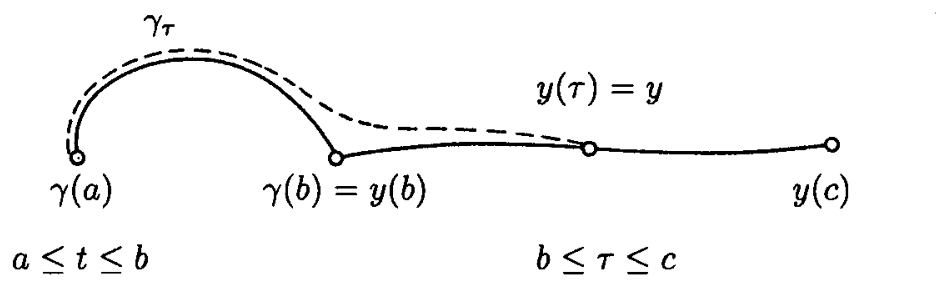
\includegraphics[width=0.78\textwidth]{figures/fig2_4.png}
  \figtitle{2.4}{}
\end{figure}
在此例中，全空间 $X$ 包含空间 $B$ 的一个嵌入副本，由常道路 $\gamma(t)\equiv\text{const.}$ 组成，因此可以把 $B$ 与它等同。容易看出，这个子空间 $B$ 是 $X$ 的形变收缩。特别重要的是 $B$ 为单点 $\{y_0\}$（$y_0\in Y$）的情形；此时空间 $X$ 可缩。在这种情形下 $X$ 通常记作 $E_{y_0}$，而 $y\in Y$ 上的纤维 $F_y$ 记作 $\Omega(y_0,y)$。（正如前面在更一般的框架下指出过的，只要底空间 $Y$ 道路连通，诸纤维 $\Omega(y_0,y)$ 就都有相同的同伦型。）对 $y=y_0$，空间 $\Omega(y_0,y_0)=\Omega$ 就是 $Y$ 的以 $y_0$ 为基点的\emph{环路空间}。
% [Tutor Note: $\Omega(y_0,y)$ 是「从 $y_0$ 到 $y$ 的道路」构成的空间，$\Omega(y_0,y_0)=\Omega$ 是闭道路（环路）空间，即 $\Omega Y$。这个构造是第 3 章 §7 里 $\Omega$ 与悬挂 $\Sigma$ 的伴随关系、以及环路空间同调计算的出发点。]

\para{3. 局部平凡纤维化} 对\emph{局部平凡纤维化}（或\emph{纤维丛}），覆叠同伦性质建立起来要困难一些。对这类纤维化 $p:X\to Y$，所有纤维 $F_y$ 实际上都同胚于一个空间 $F$。定义条件如下：要求——与覆叠空间的情形类似——底空间 $Y$ 的每个点 $y$ 都有邻域 $U$（$y\in U\subset Y$），其
% CHUNK ch02a DONE
